\documentclass{article}
\usepackage{times}
\usepackage[letterpaper, textwidth=5.5in]{geometry}  % ICLR text width
\usepackage{pgfplots}
\pgfplotsset{compat=1.17}
\providecommand{\satprob}{\mathrm{Pr}}
\providecommand{\X}{\mathcal{X}}
\begin{document}
\begin{center}% Generated by ICLR_Q4.py -- shared legend for the Q4 plots. Requires \usepackage{pgfplots}.
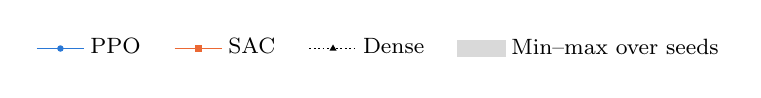
\begin{tikzpicture}
\definecolor{q4ppo}{RGB}{42,120,214}
\definecolor{q4sac}{RGB}{235,104,52}
\definecolor{q4dense}{RGB}{0,0,0}
\begin{axis}[
    hide axis, scale only axis, width=1pt, height=1pt, xmin=0, xmax=1, ymin=0, ymax=1,
    legend columns=-1, legend style={draw=none, font=\footnotesize, at={(0.5,0.5)}, anchor=center,
        /tikz/every even column/.append style={column sep=1em}},
]
\addlegendimage{q4ppo, semithick, mark=*, mark size=0.85pt}
\addlegendentry{PPO}
\addlegendimage{q4sac, semithick, mark=square*, mark size=0.85pt}
\addlegendentry{SAC}
\addlegendimage{q4dense, semithick, mark=triangle*, mark size=0.85pt, densely dotted, mark options={solid}}
\addlegendentry{Dense}
\addlegendimage{area legend, draw=gray!30, fill=gray!30}
\addlegendentry{Min--max over seeds}
\end{axis}
\end{tikzpicture}%
\end{center}
\section*{Drone4D\_x0set}
\noindent
\begin{minipage}[b]{0.24\textwidth}% Generated by ICLR_Q4.py from experiment_logs_Q4 -- Drone4D_x0set: Reach-avoid prob.
% Shaded band = min/max over seeds; line = median over seeds.
% Picture width is exactly \linewidth. Requires \usepackage{pgfplots}.
% Bounds below ymin lie outside the axis range and are clipped.
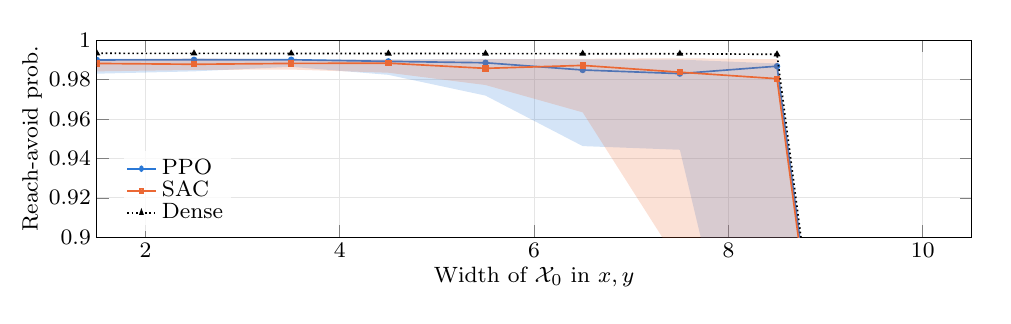
\begin{tikzpicture}[baseline=(current axis.south)]
\definecolor{q4ppo}{RGB}{42,120,214}
\definecolor{q4sac}{RGB}{235,104,52}
\definecolor{q4dense}{RGB}{0,0,0}
\begin{axis}[
    scale only axis, width=\linewidth-25pt-4pt, height=2.5cm,
    xlabel={Width of $\X_0$ in $x,y$},
    ylabel={Reach-avoid prob.}, ylabel style={align=center},
    xmin=1.5, xmax=10.5, xtick={2,4,6,8,10},
    ymin=0.9, ymax=1,
    grid=major, grid style={gray!20}, clip marker paths=true,
    label style={font=\footnotesize}, tick label style={font=\footnotesize, inner sep=2pt},
    xlabel shift=-2pt, ylabel shift=-3pt,  % labels close to the tick labels
    legend pos=south west, legend cell align=left,
    legend style={font=\footnotesize, draw=none, fill=white, fill opacity=0.8, text opacity=1,
        inner sep=1pt, row sep=-3pt},
    legend image post style={xscale=0.6},
]
% PPO: 5 seeds per X0 span
\addplot[draw=none, fill=q4ppo, fill opacity=0.2, forget plot] coordinates {(1.5,0.983048) (2.5,0.984237) (3.5,0.986539) (4.5,0.982462) (5.5,0.971915) (6.5,0.946265) (7.5,0.944395) (8.5,0.737561) (9.5,0.579626) (10.5,6.47648e-05) (10.5,6.60345e-05) (9.5,0.615019) (8.5,0.98822) (7.5,0.990203) (6.5,0.990298) (5.5,0.99061) (4.5,0.990302) (3.5,0.990244) (2.5,0.990682) (1.5,0.99063)} -- cycle;
\addplot[q4ppo, semithick, mark=*, mark size=0.85pt] coordinates {(1.5,0.990029) (2.5,0.990095) (3.5,0.990135) (4.5,0.989302) (5.5,0.988594) (6.5,0.984926) (7.5,0.983088) (8.5,0.986856) (9.5,0.614088) (10.5,6.59718e-05)};
\addlegendentry{PPO}
% SAC: 5 seeds per X0 span
\addplot[draw=none, fill=q4sac, fill opacity=0.2, forget plot] coordinates {(1.5,0.984227) (2.5,0.984956) (3.5,0.98514) (4.5,0.983544) (5.5,0.977283) (6.5,0.963407) (7.5,0.885949) (8.5,0.224063) (9.5,0.010669) (10.5,0) (10.5,6.60885e-05) (9.5,0.615674) (8.5,0.99041) (7.5,0.990888) (6.5,0.990597) (5.5,0.990402) (4.5,0.990131) (3.5,0.990286) (2.5,0.990748) (1.5,0.990256)} -- cycle;
\addplot[q4sac, semithick, mark=square*, mark size=0.85pt] coordinates {(1.5,0.988244) (2.5,0.987828) (3.5,0.988263) (4.5,0.988385) (5.5,0.985761) (6.5,0.987255) (7.5,0.983802) (8.5,0.980507) (9.5,0.613256) (10.5,6.57905e-05)};
\addlegendentry{SAC}
% Dense (single deterministic run per X0 span)
\addplot[q4dense, semithick, mark=triangle*, mark size=0.85pt, densely dotted, mark options={solid}] coordinates {(1.5,0.993398) (2.5,0.993361) (3.5,0.993323) (4.5,0.993289) (5.5,0.993252) (6.5,0.993215) (7.5,0.993182) (8.5,0.992878) (9.5,0.616133) (10.5,6.6147e-05)};
\addlegendentry{Dense}
\end{axis}
% Fix the bounding box to exactly \linewidth wide: the axis box plus the label margins
\path (current axis.south west |- current bounding box.south) ++(-25pt,0) coordinate (q4sw)
      (current axis.north east |- current bounding box.north) ++(4pt,0) coordinate (q4ne);
\pgfresetboundingbox
\useasboundingbox (q4sw) rectangle (q4ne);
\end{tikzpicture}%
\end{minipage}\hfill
\begin{minipage}[b]{0.24\textwidth}% Generated by ICLR_Q4.py from experiment_logs_Q4 -- Drone4D_x0set: Reach-avoid prob.
% Shaded band = min/max over seeds; line = median over seeds.
% Picture width is exactly \linewidth. Requires \usepackage{pgfplots}.
% Broken y axis: 0-0.9 fills the bottom half of the plot, 0.9-1 the top half.
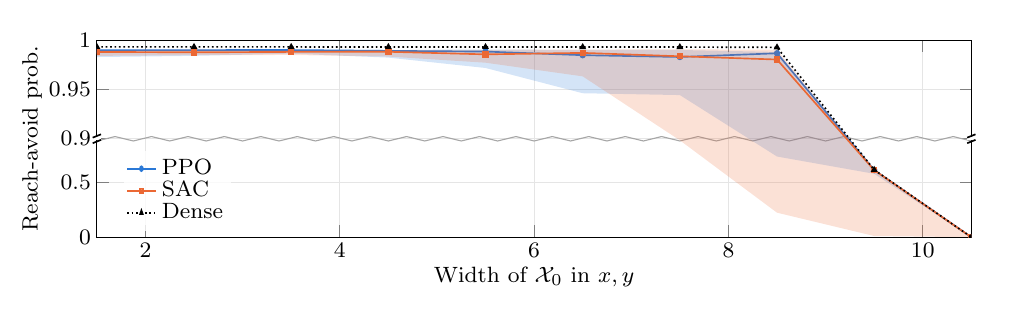
\begin{tikzpicture}[baseline=(current axis.south)]
\definecolor{q4ppo}{RGB}{42,120,214}
\definecolor{q4sac}{RGB}{235,104,52}
\definecolor{q4dense}{RGB}{0,0,0}
\begin{axis}[
    scale only axis, width=\linewidth-25pt-4pt, height=2.5cm,
    xlabel={Width of $\X_0$ in $x,y$},
    ylabel={Reach-avoid prob.}, ylabel style={align=center},
    xmin=1.5, xmax=10.5, xtick={2,4,6,8,10},
    ymin=0, ymax=1, ytick={0,0.5,0.9,0.95,1}, yticklabels={0,0.5,0.9,0.95,1},
    grid=major, grid style={gray!20}, clip marker paths=true,
    label style={font=\footnotesize}, tick label style={font=\footnotesize, inner sep=2pt},
    xlabel shift=-2pt, ylabel shift=-3pt,  % labels close to the tick labels
    y coord trafo/.code={\pgfmathparse{#1 < 0.9 ? #1*0.555556 : 0.5 + (#1 - 0.9)*5}},
    y coord inv trafo/.code={\pgfmathparse{#1 < 0.5 ? #1/0.555556 : 0.9 + (#1 - 0.5)/5}},
    legend pos=south west, legend cell align=left,
    legend style={font=\footnotesize, draw=none, fill=white, fill opacity=0.8, text opacity=1,
        inner sep=1pt, row sep=-3pt},
    legend image post style={xscale=0.6},
]
% Zigzag line across the plot at 0.9, where the y scale changes (drawn below the data)
\draw[gray!70, thin, line join=round] ([yshift=-0.8pt]rel axis cs:0,0.5) -- ([yshift=0.8pt]rel axis cs:0.02083,0.5) -- ([yshift=-0.8pt]rel axis cs:0.04167,0.5) -- ([yshift=0.8pt]rel axis cs:0.0625,0.5) -- ([yshift=-0.8pt]rel axis cs:0.08333,0.5) -- ([yshift=0.8pt]rel axis cs:0.1042,0.5) -- ([yshift=-0.8pt]rel axis cs:0.125,0.5) -- ([yshift=0.8pt]rel axis cs:0.1458,0.5) -- ([yshift=-0.8pt]rel axis cs:0.1667,0.5) -- ([yshift=0.8pt]rel axis cs:0.1875,0.5) -- ([yshift=-0.8pt]rel axis cs:0.2083,0.5) -- ([yshift=0.8pt]rel axis cs:0.2292,0.5) -- ([yshift=-0.8pt]rel axis cs:0.25,0.5) -- ([yshift=0.8pt]rel axis cs:0.2708,0.5) -- ([yshift=-0.8pt]rel axis cs:0.2917,0.5) -- ([yshift=0.8pt]rel axis cs:0.3125,0.5) -- ([yshift=-0.8pt]rel axis cs:0.3333,0.5) -- ([yshift=0.8pt]rel axis cs:0.3542,0.5) -- ([yshift=-0.8pt]rel axis cs:0.375,0.5) -- ([yshift=0.8pt]rel axis cs:0.3958,0.5) -- ([yshift=-0.8pt]rel axis cs:0.4167,0.5) -- ([yshift=0.8pt]rel axis cs:0.4375,0.5) -- ([yshift=-0.8pt]rel axis cs:0.4583,0.5) -- ([yshift=0.8pt]rel axis cs:0.4792,0.5) -- ([yshift=-0.8pt]rel axis cs:0.5,0.5) -- ([yshift=0.8pt]rel axis cs:0.5208,0.5) -- ([yshift=-0.8pt]rel axis cs:0.5417,0.5) -- ([yshift=0.8pt]rel axis cs:0.5625,0.5) -- ([yshift=-0.8pt]rel axis cs:0.5833,0.5) -- ([yshift=0.8pt]rel axis cs:0.6042,0.5) -- ([yshift=-0.8pt]rel axis cs:0.625,0.5) -- ([yshift=0.8pt]rel axis cs:0.6458,0.5) -- ([yshift=-0.8pt]rel axis cs:0.6667,0.5) -- ([yshift=0.8pt]rel axis cs:0.6875,0.5) -- ([yshift=-0.8pt]rel axis cs:0.7083,0.5) -- ([yshift=0.8pt]rel axis cs:0.7292,0.5) -- ([yshift=-0.8pt]rel axis cs:0.75,0.5) -- ([yshift=0.8pt]rel axis cs:0.7708,0.5) -- ([yshift=-0.8pt]rel axis cs:0.7917,0.5) -- ([yshift=0.8pt]rel axis cs:0.8125,0.5) -- ([yshift=-0.8pt]rel axis cs:0.8333,0.5) -- ([yshift=0.8pt]rel axis cs:0.8542,0.5) -- ([yshift=-0.8pt]rel axis cs:0.875,0.5) -- ([yshift=0.8pt]rel axis cs:0.8958,0.5) -- ([yshift=-0.8pt]rel axis cs:0.9167,0.5) -- ([yshift=0.8pt]rel axis cs:0.9375,0.5) -- ([yshift=-0.8pt]rel axis cs:0.9583,0.5) -- ([yshift=0.8pt]rel axis cs:0.9792,0.5) -- ([yshift=-0.8pt]rel axis cs:1,0.5);
% PPO: 5 seeds per X0 span
\addplot[draw=none, fill=q4ppo, fill opacity=0.2, forget plot] coordinates {(1.5,0.983048) (2.5,0.984237) (3.5,0.986539) (4.5,0.982462) (5.5,0.971915) (6.5,0.946265) (7.5,0.944395) (8.5,0.737561) (9.5,0.579626) (10.5,6.47648e-05) (10.5,6.60345e-05) (9.5,0.615019) (8.5,0.98822) (7.5,0.990203) (6.5,0.990298) (5.5,0.99061) (4.5,0.990302) (3.5,0.990244) (2.5,0.990682) (1.5,0.99063)} -- cycle;
\addplot[q4ppo, semithick, mark=*, mark size=0.85pt] coordinates {(1.5,0.990029) (2.5,0.990095) (3.5,0.990135) (4.5,0.989302) (5.5,0.988594) (6.5,0.984926) (7.5,0.983088) (8.5,0.986856) (9.5,0.614088) (10.5,6.59718e-05)};
\addlegendentry{PPO}
% SAC: 5 seeds per X0 span
\addplot[draw=none, fill=q4sac, fill opacity=0.2, forget plot] coordinates {(1.5,0.984227) (2.5,0.984956) (3.5,0.98514) (4.5,0.983544) (5.5,0.977283) (6.5,0.963407) (7.5,0.885949) (8.5,0.224063) (9.5,0.010669) (10.5,0) (10.5,6.60885e-05) (9.5,0.615674) (8.5,0.99041) (7.5,0.990888) (6.5,0.990597) (5.5,0.990402) (4.5,0.990131) (3.5,0.990286) (2.5,0.990748) (1.5,0.990256)} -- cycle;
\addplot[q4sac, semithick, mark=square*, mark size=0.85pt] coordinates {(1.5,0.988244) (2.5,0.987828) (3.5,0.988263) (4.5,0.988385) (5.5,0.985761) (6.5,0.987255) (7.5,0.983802) (8.5,0.980507) (9.5,0.613256) (10.5,6.57905e-05)};
\addlegendentry{SAC}
% Dense (single deterministic run per X0 span)
\addplot[q4dense, semithick, mark=triangle*, mark size=0.85pt, densely dotted, mark options={solid}] coordinates {(1.5,0.993398) (2.5,0.993361) (3.5,0.993323) (4.5,0.993289) (5.5,0.993252) (6.5,0.993215) (7.5,0.993182) (8.5,0.992878) (9.5,0.616133) (10.5,6.6147e-05)};
\addlegendentry{Dense}
\end{axis}
% Break marks on both sides of the y axis at 0.9, where the scale changes
\path (current axis.south west) -- (current axis.north west) coordinate[pos=0.5] (q4brkW);
\path (current axis.south east) -- (current axis.north east) coordinate[pos=0.5] (q4brkE);
\foreach \p in {q4brkW, q4brkE} {
    \fill[white] ([xshift=-1.5pt, yshift=-0.6pt]\p) rectangle ([xshift=1.5pt, yshift=0.6pt]\p);
    \draw[semithick] ([xshift=-1.5pt, yshift=-1.6pt]\p) -- ([xshift=1.5pt, yshift=-0.4pt]\p)
                     ([xshift=-1.5pt, yshift=0.4pt]\p) -- ([xshift=1.5pt, yshift=1.6pt]\p);
}
% Fix the bounding box to exactly \linewidth wide: the axis box plus the label margins
\path (current axis.south west |- current bounding box.south) ++(-25pt,0) coordinate (q4sw)
      (current axis.north east |- current bounding box.north) ++(4pt,0) coordinate (q4ne);
\pgfresetboundingbox
\useasboundingbox (q4sw) rectangle (q4ne);
\end{tikzpicture}%
\end{minipage}\hfill
\begin{minipage}[b]{0.24\textwidth}% Generated by ICLR_Q4.py from experiment_logs_Q4 -- Drone4D_x0set: Total runtime [s]
% Shaded band = min/max over seeds; line = median over seeds.
% Picture width is exactly \linewidth. Requires \usepackage{pgfplots}.
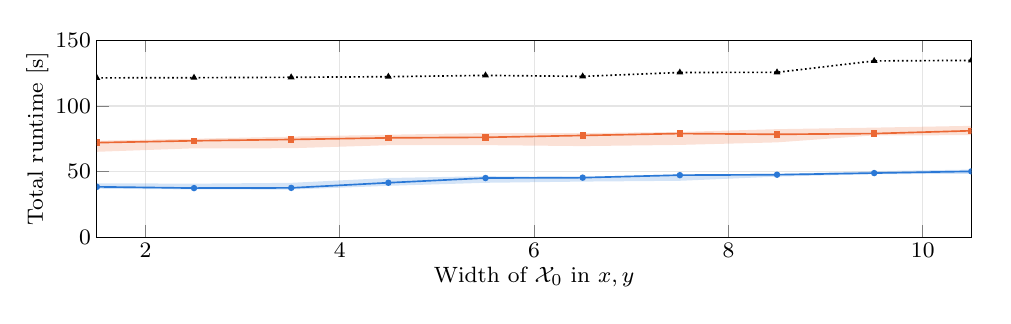
\begin{tikzpicture}[baseline=(current axis.south)]
\definecolor{q4ppo}{RGB}{42,120,214}
\definecolor{q4sac}{RGB}{235,104,52}
\definecolor{q4dense}{RGB}{0,0,0}
\begin{axis}[
    scale only axis, width=\linewidth-25pt-4pt, height=2.5cm,
    xlabel={Width of $\X_0$ in $x,y$},
    ylabel={Total runtime [s]}, ylabel style={align=center},
    xmin=1.5, xmax=10.5, xtick={2,4,6,8,10},
    ymin=0, ymax=150, ytick={0,50,100,150},
    grid=major, grid style={gray!20}, clip marker paths=true,
    label style={font=\footnotesize}, tick label style={font=\footnotesize, inner sep=2pt},
    xlabel shift=-2pt, ylabel shift=-3pt,  % labels close to the tick labels
]
% PPO: 5 seeds per X0 span
\addplot[draw=none, fill=q4ppo, fill opacity=0.2, forget plot] coordinates {(1.5,36.943) (2.5,36.4193) (3.5,36.2862) (4.5,39.1303) (5.5,41.4421) (6.5,42.3687) (7.5,42.9795) (8.5,46.1563) (9.5,48.0422) (10.5,48.3178) (10.5,51.5103) (9.5,50.3494) (8.5,48.2333) (7.5,47.9066) (6.5,45.9376) (5.5,46.4973) (4.5,45.0999) (3.5,41.4188) (2.5,40.7996) (1.5,41.106)} -- cycle;
\addplot[q4ppo, semithick, mark=*, mark size=0.85pt] coordinates {(1.5,38.3778) (2.5,37.4156) (3.5,37.5686) (4.5,41.492) (5.5,45.081) (6.5,45.3668) (7.5,47.2769) (8.5,47.6097) (9.5,48.8671) (10.5,50.1497)};
% SAC: 5 seeds per X0 span
\addplot[draw=none, fill=q4sac, fill opacity=0.2, forget plot] coordinates {(1.5,65.0665) (2.5,67.7267) (3.5,67.7845) (4.5,70.1071) (5.5,70.1528) (6.5,69.4144) (7.5,70.3135) (8.5,72.2586) (9.5,77.5874) (10.5,77.7245) (10.5,84.8415) (9.5,83.4859) (8.5,82.3169) (7.5,80.1923) (6.5,79.3013) (5.5,79.3646) (4.5,78.0795) (3.5,76.6222) (2.5,75.035) (1.5,73.5015)} -- cycle;
\addplot[q4sac, semithick, mark=square*, mark size=0.85pt] coordinates {(1.5,72.0344) (2.5,73.461) (3.5,74.4472) (4.5,75.6932) (5.5,76.0961) (6.5,77.5104) (7.5,78.9612) (8.5,78.3844) (9.5,78.9615) (10.5,81.1042)};
% Dense (single deterministic run per X0 span)
\addplot[q4dense, semithick, mark=triangle*, mark size=0.85pt, densely dotted, mark options={solid}] coordinates {(1.5,121.39) (2.5,121.538) (3.5,121.833) (4.5,122.307) (5.5,123.286) (6.5,122.546) (7.5,125.505) (8.5,125.631) (9.5,134.307) (10.5,134.718)};
\end{axis}
% Fix the bounding box to exactly \linewidth wide: the axis box plus the label margins
\path (current axis.south west |- current bounding box.south) ++(-25pt,0) coordinate (q4sw)
      (current axis.north east |- current bounding box.north) ++(4pt,0) coordinate (q4ne);
\pgfresetboundingbox
\useasboundingbox (q4sw) rectangle (q4ne);
\end{tikzpicture}%
\end{minipage}\hfill
\begin{minipage}[b]{0.24\textwidth}% Generated by ICLR_Q4.py from experiment_logs_Q4 -- Drone4D_x0set: Abstract states ($|S|$)
% Shaded band = min/max over seeds; line = median over seeds.
% Picture width is exactly \linewidth. Requires \usepackage{pgfplots}.
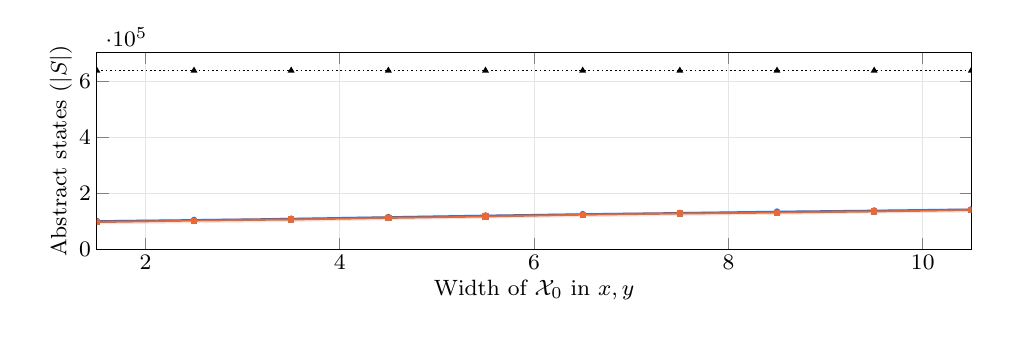
\begin{tikzpicture}[baseline=(current axis.south)]
\definecolor{q4ppo}{RGB}{42,120,214}
\definecolor{q4sac}{RGB}{235,104,52}
\definecolor{q4dense}{RGB}{0,0,0}
\begin{axis}[
    scale only axis, width=\linewidth-25pt-4pt, height=2.5cm,
    xlabel={Width of $\X_0$ in $x,y$},
    ylabel={Abstract states ($|S|$)}, ylabel style={align=center},
    xmin=1.5, xmax=10.5, xtick={2,4,6,8,10},
    ymin=0,
    grid=major, grid style={gray!20}, clip marker paths=true,
    label style={font=\footnotesize}, tick label style={font=\footnotesize, inner sep=2pt},
    xlabel shift=-2pt, ylabel shift=-3pt,  % labels close to the tick labels
]
% PPO: 5 seeds per X0 span
\addplot[draw=none, fill=q4ppo, fill opacity=0.2, forget plot] coordinates {(1.5,98744) (2.5,103375) (3.5,107424) (4.5,112760) (5.5,119166) (6.5,124791) (7.5,129688) (8.5,132625) (9.5,137618) (10.5,142700) (10.5,147256) (9.5,142704) (8.5,138887) (7.5,135526) (6.5,130372) (5.5,125180) (4.5,119773) (3.5,114423) (2.5,109788) (1.5,105379)} -- cycle;
\addplot[q4ppo, semithick, mark=*, mark size=0.85pt] coordinates {(1.5,101852) (2.5,105732) (3.5,110207) (4.5,116071) (5.5,121652) (6.5,126682) (7.5,130994) (8.5,135769) (9.5,139486) (10.5,143836)};
% SAC: 5 seeds per X0 span
\addplot[draw=none, fill=q4sac, fill opacity=0.2, forget plot] coordinates {(1.5,89969) (2.5,94202) (3.5,98888) (4.5,104859) (5.5,110774) (6.5,115750) (7.5,120421) (8.5,124158) (9.5,128485) (10.5,132828) (10.5,144613) (9.5,139754) (8.5,135710) (7.5,131505) (6.5,127182) (5.5,122306) (4.5,115567) (3.5,110532) (2.5,105015) (1.5,101244)} -- cycle;
\addplot[q4sac, semithick, mark=square*, mark size=0.85pt] coordinates {(1.5,97565) (2.5,102945) (3.5,106818) (4.5,112453) (5.5,117588) (6.5,123979) (7.5,128151) (8.5,131569) (9.5,135548) (10.5,140717)};
% Dense (single deterministic run per X0 span)
\addplot[q4dense, semithick, mark=triangle*, mark size=0.85pt, densely dotted, mark options={solid}] coordinates {(1.5,640000) (2.5,640000) (3.5,640000) (4.5,640000) (5.5,640000) (6.5,640000) (7.5,640000) (8.5,640000) (9.5,640000) (10.5,640000)};
\end{axis}
% Fix the bounding box to exactly \linewidth wide: the axis box plus the label margins
\path (current axis.south west |- current bounding box.south) ++(-25pt,0) coordinate (q4sw)
      (current axis.north east |- current bounding box.north) ++(4pt,0) coordinate (q4ne);
\pgfresetboundingbox
\useasboundingbox (q4sw) rectangle (q4ne);
\end{tikzpicture}%
\end{minipage}\hfill

\section*{Dubins4D\_x0set}
\noindent
\begin{minipage}[b]{0.24\textwidth}% Generated by ICLR_Q4.py from experiment_logs_Q4 -- Dubins4D_x0set: Reach-avoid prob.
% Shaded band = min/max over seeds; line = median over seeds.
% Picture width is exactly \linewidth. Requires \usepackage{pgfplots}.
% Bounds below ymin lie outside the axis range and are clipped.
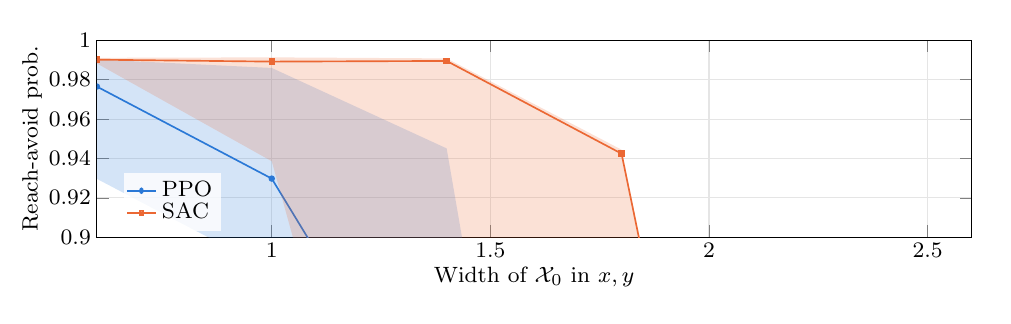
\begin{tikzpicture}[baseline=(current axis.south)]
\definecolor{q4ppo}{RGB}{42,120,214}
\definecolor{q4sac}{RGB}{235,104,52}
\begin{axis}[
    scale only axis, width=\linewidth-25pt-4pt, height=2.5cm,
    xlabel={Width of $\X_0$ in $x,y$},
    ylabel={Reach-avoid prob.}, ylabel style={align=center},
    xmin=0.6, xmax=2.6, xtick={1,1.5,2,2.5},
    ymin=0.9, ymax=1,
    grid=major, grid style={gray!20}, clip marker paths=true,
    label style={font=\footnotesize}, tick label style={font=\footnotesize, inner sep=2pt},
    xlabel shift=-2pt, ylabel shift=-3pt,  % labels close to the tick labels
    legend pos=south west, legend cell align=left,
    legend style={font=\footnotesize, draw=none, fill=white, fill opacity=0.8, text opacity=1,
        inner sep=1pt, row sep=-3pt},
    legend image post style={xscale=0.6},
]
% PPO: 5 seeds per X0 span
\addplot[draw=none, fill=q4ppo, fill opacity=0.2, forget plot] coordinates {(0.6,0.929625) (1,0.882996) (1.4,0.742007) (1.8,0.259818) (2.2,0.0022184) (2.6,7.25751e-08) (2.6,7.41889e-06) (2.2,0.0575252) (1.8,0.430475) (1.4,0.945096) (1,0.985959) (0.6,0.990287)} -- cycle;
\addplot[q4ppo, semithick, mark=*, mark size=0.85pt] coordinates {(0.6,0.976511) (1,0.929754) (1.4,0.783714) (1.8,0.280157) (2.2,0.00795742) (2.6,3.39054e-07)};
\addlegendentry{PPO}
% SAC: 2/5 seeds per X0 span
\addplot[draw=none, fill=q4sac, fill opacity=0.2, forget plot] coordinates {(0.6,0.988255) (1,0.938558) (1.4,0.619015) (1.8,0.100169) (2.2,0.00122616) (2.6,0) (2.6,0.0328988) (2.2,0.513128) (1.8,0.944437) (1.4,0.990815) (1,0.991339) (0.6,0.991103)} -- cycle;
\addplot[q4sac, semithick, mark=square*, mark size=0.85pt] coordinates {(0.6,0.990163) (1,0.989182) (1.4,0.989519) (1.8,0.942418) (2.2,0.512191) (2.6,0.0164494)};
\addlegendentry{SAC}
\end{axis}
% Fix the bounding box to exactly \linewidth wide: the axis box plus the label margins
\path (current axis.south west |- current bounding box.south) ++(-25pt,0) coordinate (q4sw)
      (current axis.north east |- current bounding box.north) ++(4pt,0) coordinate (q4ne);
\pgfresetboundingbox
\useasboundingbox (q4sw) rectangle (q4ne);
\end{tikzpicture}%
\end{minipage}\hfill
\begin{minipage}[b]{0.24\textwidth}% Generated by ICLR_Q4.py from experiment_logs_Q4 -- Dubins4D_x0set: Reach-avoid prob.
% Shaded band = min/max over seeds; line = median over seeds.
% Picture width is exactly \linewidth. Requires \usepackage{pgfplots}.
% Broken y axis: 0-0.9 fills the bottom half of the plot, 0.9-1 the top half.
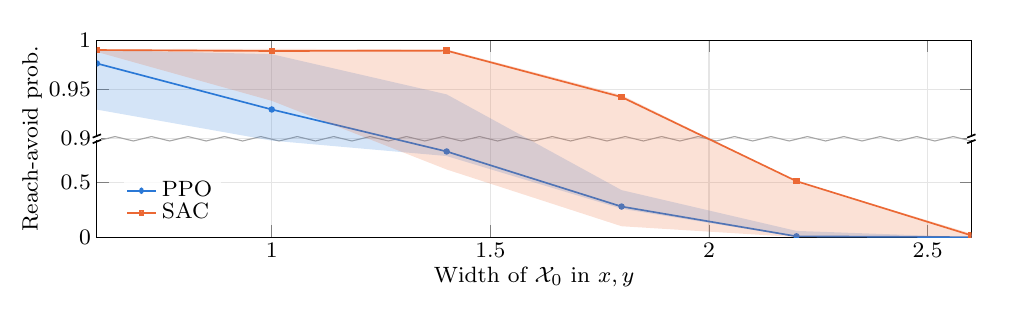
\begin{tikzpicture}[baseline=(current axis.south)]
\definecolor{q4ppo}{RGB}{42,120,214}
\definecolor{q4sac}{RGB}{235,104,52}
\begin{axis}[
    scale only axis, width=\linewidth-25pt-4pt, height=2.5cm,
    xlabel={Width of $\X_0$ in $x,y$},
    ylabel={Reach-avoid prob.}, ylabel style={align=center},
    xmin=0.6, xmax=2.6, xtick={1,1.5,2,2.5},
    ymin=0, ymax=1, ytick={0,0.5,0.9,0.95,1}, yticklabels={0,0.5,0.9,0.95,1},
    grid=major, grid style={gray!20}, clip marker paths=true,
    label style={font=\footnotesize}, tick label style={font=\footnotesize, inner sep=2pt},
    xlabel shift=-2pt, ylabel shift=-3pt,  % labels close to the tick labels
    y coord trafo/.code={\pgfmathparse{#1 < 0.9 ? #1*0.555556 : 0.5 + (#1 - 0.9)*5}},
    y coord inv trafo/.code={\pgfmathparse{#1 < 0.5 ? #1/0.555556 : 0.9 + (#1 - 0.5)/5}},
    legend pos=south west, legend cell align=left,
    legend style={font=\footnotesize, draw=none, fill=white, fill opacity=0.8, text opacity=1,
        inner sep=1pt, row sep=-3pt},
    legend image post style={xscale=0.6},
]
% Zigzag line across the plot at 0.9, where the y scale changes (drawn below the data)
\draw[gray!70, thin, line join=round] ([yshift=-0.8pt]rel axis cs:0,0.5) -- ([yshift=0.8pt]rel axis cs:0.02083,0.5) -- ([yshift=-0.8pt]rel axis cs:0.04167,0.5) -- ([yshift=0.8pt]rel axis cs:0.0625,0.5) -- ([yshift=-0.8pt]rel axis cs:0.08333,0.5) -- ([yshift=0.8pt]rel axis cs:0.1042,0.5) -- ([yshift=-0.8pt]rel axis cs:0.125,0.5) -- ([yshift=0.8pt]rel axis cs:0.1458,0.5) -- ([yshift=-0.8pt]rel axis cs:0.1667,0.5) -- ([yshift=0.8pt]rel axis cs:0.1875,0.5) -- ([yshift=-0.8pt]rel axis cs:0.2083,0.5) -- ([yshift=0.8pt]rel axis cs:0.2292,0.5) -- ([yshift=-0.8pt]rel axis cs:0.25,0.5) -- ([yshift=0.8pt]rel axis cs:0.2708,0.5) -- ([yshift=-0.8pt]rel axis cs:0.2917,0.5) -- ([yshift=0.8pt]rel axis cs:0.3125,0.5) -- ([yshift=-0.8pt]rel axis cs:0.3333,0.5) -- ([yshift=0.8pt]rel axis cs:0.3542,0.5) -- ([yshift=-0.8pt]rel axis cs:0.375,0.5) -- ([yshift=0.8pt]rel axis cs:0.3958,0.5) -- ([yshift=-0.8pt]rel axis cs:0.4167,0.5) -- ([yshift=0.8pt]rel axis cs:0.4375,0.5) -- ([yshift=-0.8pt]rel axis cs:0.4583,0.5) -- ([yshift=0.8pt]rel axis cs:0.4792,0.5) -- ([yshift=-0.8pt]rel axis cs:0.5,0.5) -- ([yshift=0.8pt]rel axis cs:0.5208,0.5) -- ([yshift=-0.8pt]rel axis cs:0.5417,0.5) -- ([yshift=0.8pt]rel axis cs:0.5625,0.5) -- ([yshift=-0.8pt]rel axis cs:0.5833,0.5) -- ([yshift=0.8pt]rel axis cs:0.6042,0.5) -- ([yshift=-0.8pt]rel axis cs:0.625,0.5) -- ([yshift=0.8pt]rel axis cs:0.6458,0.5) -- ([yshift=-0.8pt]rel axis cs:0.6667,0.5) -- ([yshift=0.8pt]rel axis cs:0.6875,0.5) -- ([yshift=-0.8pt]rel axis cs:0.7083,0.5) -- ([yshift=0.8pt]rel axis cs:0.7292,0.5) -- ([yshift=-0.8pt]rel axis cs:0.75,0.5) -- ([yshift=0.8pt]rel axis cs:0.7708,0.5) -- ([yshift=-0.8pt]rel axis cs:0.7917,0.5) -- ([yshift=0.8pt]rel axis cs:0.8125,0.5) -- ([yshift=-0.8pt]rel axis cs:0.8333,0.5) -- ([yshift=0.8pt]rel axis cs:0.8542,0.5) -- ([yshift=-0.8pt]rel axis cs:0.875,0.5) -- ([yshift=0.8pt]rel axis cs:0.8958,0.5) -- ([yshift=-0.8pt]rel axis cs:0.9167,0.5) -- ([yshift=0.8pt]rel axis cs:0.9375,0.5) -- ([yshift=-0.8pt]rel axis cs:0.9583,0.5) -- ([yshift=0.8pt]rel axis cs:0.9792,0.5) -- ([yshift=-0.8pt]rel axis cs:1,0.5);
% PPO: 5 seeds per X0 span
\addplot[draw=none, fill=q4ppo, fill opacity=0.2, forget plot] coordinates {(0.6,0.929625) (1,0.882996) (1.4,0.742007) (1.8,0.259818) (2.2,0.0022184) (2.6,7.25751e-08) (2.6,7.41889e-06) (2.2,0.0575252) (1.8,0.430475) (1.4,0.945096) (1,0.985959) (0.6,0.990287)} -- cycle;
\addplot[q4ppo, semithick, mark=*, mark size=0.85pt] coordinates {(0.6,0.976511) (1,0.929754) (1.4,0.783714) (1.8,0.280157) (2.2,0.00795742) (2.6,3.39054e-07)};
\addlegendentry{PPO}
% SAC: 2/5 seeds per X0 span
\addplot[draw=none, fill=q4sac, fill opacity=0.2, forget plot] coordinates {(0.6,0.988255) (1,0.938558) (1.4,0.619015) (1.8,0.100169) (2.2,0.00122616) (2.6,0) (2.6,0.0328988) (2.2,0.513128) (1.8,0.944437) (1.4,0.990815) (1,0.991339) (0.6,0.991103)} -- cycle;
\addplot[q4sac, semithick, mark=square*, mark size=0.85pt] coordinates {(0.6,0.990163) (1,0.989182) (1.4,0.989519) (1.8,0.942418) (2.2,0.512191) (2.6,0.0164494)};
\addlegendentry{SAC}
\end{axis}
% Break marks on both sides of the y axis at 0.9, where the scale changes
\path (current axis.south west) -- (current axis.north west) coordinate[pos=0.5] (q4brkW);
\path (current axis.south east) -- (current axis.north east) coordinate[pos=0.5] (q4brkE);
\foreach \p in {q4brkW, q4brkE} {
    \fill[white] ([xshift=-1.5pt, yshift=-0.6pt]\p) rectangle ([xshift=1.5pt, yshift=0.6pt]\p);
    \draw[semithick] ([xshift=-1.5pt, yshift=-1.6pt]\p) -- ([xshift=1.5pt, yshift=-0.4pt]\p)
                     ([xshift=-1.5pt, yshift=0.4pt]\p) -- ([xshift=1.5pt, yshift=1.6pt]\p);
}
% Fix the bounding box to exactly \linewidth wide: the axis box plus the label margins
\path (current axis.south west |- current bounding box.south) ++(-25pt,0) coordinate (q4sw)
      (current axis.north east |- current bounding box.north) ++(4pt,0) coordinate (q4ne);
\pgfresetboundingbox
\useasboundingbox (q4sw) rectangle (q4ne);
\end{tikzpicture}%
\end{minipage}\hfill
\begin{minipage}[b]{0.24\textwidth}% Generated by ICLR_Q4.py from experiment_logs_Q4 -- Dubins4D_x0set: Total runtime [s]
% Shaded band = min/max over seeds; line = median over seeds.
% Picture width is exactly \linewidth. Requires \usepackage{pgfplots}.
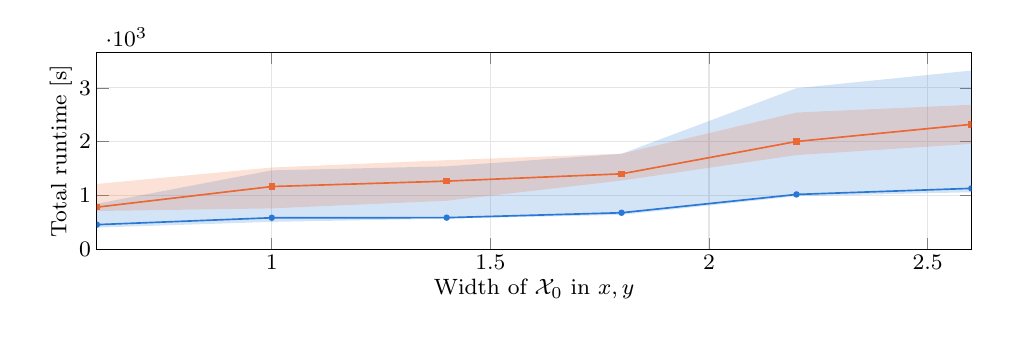
\begin{tikzpicture}[baseline=(current axis.south)]
\definecolor{q4ppo}{RGB}{42,120,214}
\definecolor{q4sac}{RGB}{235,104,52}
\begin{axis}[
    scale only axis, width=\linewidth-25pt-4pt, height=2.5cm,
    xlabel={Width of $\X_0$ in $x,y$},
    ylabel={Total runtime [s]}, ylabel style={align=center},
    xmin=0.6, xmax=2.6, xtick={1,1.5,2,2.5},
    ymin=0, scale ticks above exponent=2,
    grid=major, grid style={gray!20}, clip marker paths=true,
    label style={font=\footnotesize}, tick label style={font=\footnotesize, inner sep=2pt},
    xlabel shift=-2pt, ylabel shift=-3pt,  % labels close to the tick labels
]
% PPO: 5 seeds per X0 span
\addplot[draw=none, fill=q4ppo, fill opacity=0.2, forget plot] coordinates {(0.6,406.064) (1,512.852) (1.4,572.495) (1.8,643.146) (2.2,989.228) (2.6,1062.94) (2.6,3322.39) (2.2,2994.06) (1.8,1776.63) (1.4,1543.97) (1,1469.31) (0.6,850.361)} -- cycle;
\addplot[q4ppo, semithick, mark=*, mark size=0.85pt] coordinates {(0.6,461.161) (1,588.909) (1.4,591.171) (1.8,681.992) (2.2,1021.92) (2.6,1134.71)};
% SAC: 2/5 seeds per X0 span
\addplot[draw=none, fill=q4sac, fill opacity=0.2, forget plot] coordinates {(0.6,714.38) (1,762.866) (1.4,903.901) (1.8,1279.64) (2.2,1752.27) (2.6,1959.67) (2.6,2686.85) (2.2,2543.19) (1.8,1779.01) (1.4,1658.06) (1,1521.47) (0.6,1216.62)} -- cycle;
\addplot[q4sac, semithick, mark=square*, mark size=0.85pt] coordinates {(0.6,785.94) (1,1168.54) (1.4,1269.21) (1.8,1404.51) (2.2,2004.95) (2.6,2323.26)};
\end{axis}
% Fix the bounding box to exactly \linewidth wide: the axis box plus the label margins
\path (current axis.south west |- current bounding box.south) ++(-25pt,0) coordinate (q4sw)
      (current axis.north east |- current bounding box.north) ++(4pt,0) coordinate (q4ne);
\pgfresetboundingbox
\useasboundingbox (q4sw) rectangle (q4ne);
\end{tikzpicture}%
\end{minipage}\hfill
\begin{minipage}[b]{0.24\textwidth}% Generated by ICLR_Q4.py from experiment_logs_Q4 -- Dubins4D_x0set: Abstract states ($|S|$)
% Shaded band = min/max over seeds; line = median over seeds.
% Picture width is exactly \linewidth. Requires \usepackage{pgfplots}.
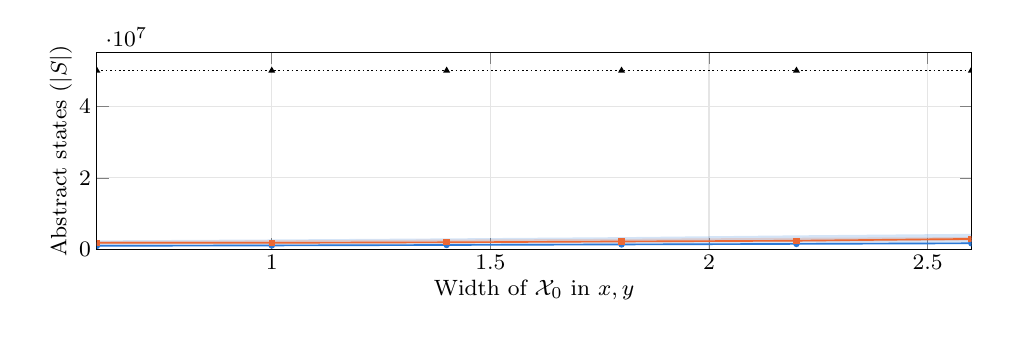
\begin{tikzpicture}[baseline=(current axis.south)]
\definecolor{q4ppo}{RGB}{42,120,214}
\definecolor{q4sac}{RGB}{235,104,52}
\definecolor{q4dense}{RGB}{0,0,0}
\begin{axis}[
    scale only axis, width=\linewidth-25pt-4pt, height=2.5cm,
    xlabel={Width of $\X_0$ in $x,y$},
    ylabel={Abstract states ($|S|$)}, ylabel style={align=center},
    xmin=0.6, xmax=2.6, xtick={1,1.5,2,2.5},
    ymin=0,
    grid=major, grid style={gray!20}, clip marker paths=true,
    label style={font=\footnotesize}, tick label style={font=\footnotesize, inner sep=2pt},
    xlabel shift=-2pt, ylabel shift=-3pt,  % labels close to the tick labels
]
% PPO: 5 seeds per X0 span
\addplot[draw=none, fill=q4ppo, fill opacity=0.2, forget plot] coordinates {(0.6,904151) (1,1.01892e+06) (1.4,1.15981e+06) (1.8,1.32139e+06) (2.2,1.50771e+06) (2.6,1.68467e+06) (2.6,4.37335e+06) (2.2,3.95113e+06) (1.8,3.45003e+06) (1.4,3.1016e+06) (1,2.79997e+06) (0.6,2.54632e+06)} -- cycle;
\addplot[q4ppo, semithick, mark=*, mark size=0.85pt] coordinates {(0.6,1.0237e+06) (1,1.13097e+06) (1.4,1.25874e+06) (1.8,1.40682e+06) (2.2,1.56507e+06) (2.6,1.73367e+06)};
% SAC: 2/5 seeds per X0 span
\addplot[draw=none, fill=q4sac, fill opacity=0.2, forget plot] coordinates {(0.6,1.56618e+06) (1,1.70914e+06) (1.4,1.81878e+06) (1.8,1.97282e+06) (2.2,2.15849e+06) (2.6,2.46615e+06) (2.6,3.46406e+06) (2.2,3.2765e+06) (1.8,2.96682e+06) (1.4,2.75992e+06) (1,2.55642e+06) (0.6,2.28302e+06)} -- cycle;
\addplot[q4sac, semithick, mark=square*, mark size=0.85pt] coordinates {(0.6,1.88455e+06) (1,1.86944e+06) (1.4,2.01058e+06) (1.8,2.24076e+06) (2.2,2.44937e+06) (2.6,2.9651e+06)};
% Dense (single deterministic run per X0 span)
% No dense run for X0 span(s) 0.6, 1, 1.4, 1.8, 2.2, 2.6: there, the number of cells of the dense grid (100x50x100x100) is plotted
\addplot[q4dense, semithick, mark=triangle*, mark size=0.85pt, densely dotted, mark options={solid}] coordinates {(0.6,5e+07) (1,5e+07) (1.4,5e+07) (1.8,5e+07) (2.2,5e+07) (2.6,5e+07)};
\end{axis}
% Fix the bounding box to exactly \linewidth wide: the axis box plus the label margins
\path (current axis.south west |- current bounding box.south) ++(-25pt,0) coordinate (q4sw)
      (current axis.north east |- current bounding box.north) ++(4pt,0) coordinate (q4ne);
\pgfresetboundingbox
\useasboundingbox (q4sw) rectangle (q4ne);
\end{tikzpicture}%
\end{minipage}\hfill

\end{document}
